
\RequirePackage{cmap}

\documentclass[
    usenatbib,
]{mnras}

\usepackage[T1]{fontenc}
\usepackage[dvipsnames, x11names]{xcolor}

\renewcommand{\baselinestretch}{1.0} % Change to 1.65 for double spacing
\usepackage{showyourwork}
\usepackage{amsmath}
\usepackage{amsfonts}
\usepackage{amssymb}
\usepackage{mathrsfs}

\usepackage{xurl}
\urlstyle{tt}

\usepackage{booktabs}
\usepackage{graphicx}
\usepackage[
    % colorlinks=true, 
    % allcolors=blue,
]{hyperref}



% Prettier fonts 
% (We might have to go back to defaults for MNRAS submission)
% \usepackage{libertine}
% \usepackage[libertine]{newtxmath}
% \usepackage[scaled=0.76]{beramono}

% Those seem to be the "right" fonts for MNRAS
\usepackage{newtxtext}
\usepackage{newtxmath}


\usepackage{microtype}
\usepackage{csquotes}
\usepackage[capitalise]{cleveref}
%\usepackage{xspace}

\usepackage{standalone}
\usepackage{tikz}
\usetikzlibrary{
    calc,
    positioning,
    shapes,
}

\usepackage{siunitx}
\sisetup{
    range-units = single,
    range-phrase = \textup{--},
    per-mode = symbol,
}
\DeclareSIUnit\parsec{pc}
\DeclareSIUnit\au{au}
\DeclareSIUnit\mas{mas}

%REMOVE LATER
\usepackage{soul}

% Load journal macros (e.g., \aa for A&A)
% Source: https://ui.adsabs.harvard.edu/help/actions/journal-macros
\usepackage{aas_macros}
% \usepackage{astro_bib_macro}  % where is this one from?

\newcommand{\todo}[1]{\textcolor{red}{[#1]}}
\newcommand{\timmy}[1]{\textcolor{red}{[\textbf{Timmy:} #1]}} % amazing

% Define macros
\newcommand{\IWA}{\ensuremath{\mathrm{IWA}}}
\newcommand{\OWA}{\ensuremath{\mathrm{OWA}}}
\newcommand{\hwo}{HabWorlds}

% Define the colors of the \rainbows
\definecolor{C0}{HTML}{ff0000}
\definecolor{C1}{HTML}{ff6d38}
\definecolor{C2}{HTML}{ecc86f}
\definecolor{C3}{HTML}{a4f89f}
\definecolor{C4}{HTML}{5af8c8}
\definecolor{C5}{HTML}{12c8e6}
\definecolor{C6}{HTML}{386df9}
\definecolor{C7}{HTML}{8000ff}

\newcommand{\rainbows}{% MAK: KEEP this formatting for MNRAS submission. It deserves this!
    \textcolor{C0}{r}%
    \textcolor{C1}{a}%
    \textcolor{C2}{i}%
    \textcolor{C3}{n}%
    \textcolor{C4}{b}%
    \textcolor{C5}{o}%
    \textcolor{C6}{w}%
    \textcolor{C7}{s}%
    % \xspace
}

% Patch \hypertarget; for details, see 
% https://tex.stackexchange.com/a/17138/97669
\makeatletter
\newcommand{\affdest}[1]{\Hy@raisedlink{\hypertarget{#1}{}}$^\mathrm{#1}$}
\makeatother
\newcommand{\afflink}[1]{\hyperlink{#1}{#1}}



% Chasing rainbows with the Habitable Worlds Observatory
\title{Chasing \rainbows{} and ocean glint:\\  Inner working angle constraints for the Habitable Worlds Observatory}

%phase angle probed by directly imaged planets, or
%Don't ask us about contrast


% Authors are in alphabetical order:
\author[Sophia R. Vaughan et al.]{%
    Sophia R. Vaughan\thanks{Correspondence:~\url{sophia.vaughan@physics.ox.ac.uk}}\textsuperscript{,\afflink{1}},
    Kimberly Bott\textsuperscript{\afflink{2},\afflink{3},\afflink{4}},
    Sarah L. Casewell\textsuperscript{\afflink{5}},
    Nicolas B. Cowan\textsuperscript{\afflink{6}},
    David S. Doelman\textsuperscript{\afflink{7},\afflink{8}},
    \newauthor
    Timothy D. Gebhard\textsuperscript{\afflink{9},\afflink{10}},
    Matthew A.  Kenworthy\textsuperscript{\afflink{7}},
    Johan Mazoyer\textsuperscript{\afflink{11}},
    Maxwell A. Millar-Blanchaer\textsuperscript{\afflink{12}},
    \newauthor
    Olivier Absil\textsuperscript{\afflink{13}},
    Lisa Altinier\textsuperscript{\afflink{14}},
    Pierre Baudoz\textsuperscript{\afflink{11}},
    Ruslan Belikov\textsuperscript{\afflink{15}},
    Alexis Bidot\textsuperscript{\afflink{16}},
    Markus J. Bonse\textsuperscript{\afflink{10}},
    \newauthor
    Bernhard Brandl\textsuperscript{\afflink{7}},
    Alexis Carlotti\textsuperscript{\afflink{16}},
    Elodie Choquet\textsuperscript{\afflink{14}},
    Niyati Desai\textsuperscript{\afflink{17}},
    Kevin Fogarty\textsuperscript{\afflink{15}},
    Jules Fowler\textsuperscript{\afflink{18}},
    \newauthor
    Yann Gutierrez\textsuperscript{\afflink{11},\afflink{19},\afflink{20}},
    Olivier Guyon\textsuperscript{\afflink{21},\afflink{22},\afflink{23},\afflink{24}},
    Sebastiaan Y. Haffert\textsuperscript{\afflink{21}},
    Olivier Herscovici-Schiller\textsuperscript{\afflink{19}},
    \newauthor
    Adrien Hours\textsuperscript{\afflink{16}},
    Roser Juanola-Parramon\textsuperscript{\afflink{25},\afflink{26}},
    Elina Kleisioti\textsuperscript{\afflink{7}},
    Lorenzo König\textsuperscript{\afflink{13}},
    Mariya Krasteva\textsuperscript{\afflink{27}},
    \newauthor
    Iva Laginja\textsuperscript{\afflink{11}},
    Rico Landman\textsuperscript{\afflink{7}},
    Lucie Leboulleux\textsuperscript{\afflink{16}},
    David Mouillet\textsuperscript{\afflink{16}},
    Mamadou N’Diaye\textsuperscript{\afflink{28}},
    \newauthor
    Emiel H. Por\textsuperscript{\afflink{29}},
    Laurent Pueyo\textsuperscript{\afflink{29}},
    Frans Snik\textsuperscript{\afflink{7}},
    Daphne M. Stam\textsuperscript{\afflink{30}},
    Victor Trees\textsuperscript{\afflink{31},\afflink{32}},
    Dirk van Dam\textsuperscript{\afflink{7}},
    \newauthor
    Kyle van Gorkom\textsuperscript{\afflink{21}},
    Maaike van Kooten\textsuperscript{\afflink{33}}
    \newauthor \\%
    Affiliations are listed at the end of the paper
    % Timmy: I checked MNRAS and it seems that this is how they handle very long author lists. See, for example:
    % https://academic.oup.com/mnras/article/498/2/2354/5900562
}
\date{Draft version: \today}


\pagestyle{plain}
 
\begin{document} 

\maketitle

\begin{abstract}
NASA recently announced the Habitable Worlds Observatory (\hwo), a coronagraphic space mission to detect rocky planets in habitable zones, establish their habitability, and search them for biosignatures. 
%Numerous instrumental and observational challenges have still to be overcome to design a coronagraphic mission with that goal. After a research phase aiming at the detection of a few tens of exo-Earth in the habitable zone, the Habitable Worlds Observatory will use its spectroscopic and polarimetric capabilities to probe these planets' atmosphere and surface properties. 
Surface liquid water is central to the definition of planetary habitability.
%
Photometric and polarimetric phase curves of starlight that is reflected by an exoplanet can reveal angular features that are due to ocean glint, and to rainbows and other phenomena caused by scattering by cloud particles. 
%
Direct imaging missions are optimised for planets near quadrature, and \hwo's coronagraph may obscure the phase angles where such characteristic features are strongest. 
%
The range of accessible phase angles for a given exoplanet will depend on the planet's orbital inclination and/or the coronagraph's inner working angle (IWA). 
%
Planets in close-to-edge-on orbits have accessible phase angles limited by coronagraph obscuration. 
%
We use the list of 160 target stars for \hwo~to estimate the number of exo-Earths that could be searched for non-Lambertian scattering phenomena. 
%
We find that any exo-Earths in systems in this catalog will have an accessible Rayleigh scattering peak in their polarimetric phase curve. 
%
The glint signature at planetary scattering angles of $\sim\qtyrange{50}{70}{\degree}$ 
%\sim$110--130$^\circ$ 
would be accessible to \hwo~in $\sim\num{14}$ systems, and the rainbow due to water clouds at phase angles of \qtyrange{140}{160}{\degree} would be accessible in $\sim\num{42}$ systems, assuming a \qty{62}{\mas} \IWA{} ($3\,\lambda/D$ for a \qty{6}{\meter} telescope at \qty{600}{\nano\meter}).
%
Increasing the \IWA{} to $2\,\lambda/D$ increases the number of systems with accessible rainbows and glints by factors of roughly 2 and 3, respectively.
%
The number of systems in which an exo-Earth could be searched for these scattering phenomena increases with the planet's orbital eccentricity and scales approximately inversely with the \IWA{}.  \end{abstract}

\begin{keywords}
planets and satellites: terrestrial planets -- 
instrumentation: high angular resolution -- 
planets and satellites: atmospheres
\end{keywords}

%%%%%%%%%%%%%%%%%%%%%%%%%%%%%%%%%%%%%%%%%%%%%%%%%%%%%%%%%%%%%%%%%%%%%%%%%%%%%%%%%

\section{Introduction}
\label{sec:intro}

%--------------------------------------------------------------------------------
%\begin{figure*}
    %\centering
    %\includegraphics[width=\linewidth]%{figures/Fig1IWAPol.png}
%    \caption{
%        The phase curves of two homogeneous planets with oceans and Earth-like atmospheres in edge-on orbits (the planets thus exhibit scattering angles 
%        ranging from 0$^\circ$ to 180$^\circ$ along their orbits). 
%        The cloudy scenario includes a low-altitude, Earth-like water 
%        cloud deck. 
%        Below the plot, we are showing the scattering angle ranges that cover the
%        characteristic features of glories, rainbows, Rayleigh scattering, glint, and forward scattering by cloud particles (note that features partly overlap
%        with each other).  
%        Throughout the paper we approximate feature sensitivity ranges as those that capture the rise and fall of peaks in polarized light for most habitable zone species in the UV, Optical, and IR (phase angles: glint $\sim\qtyrange{50}{70}{\degree}$; rainbow $\sim\SIrange{140}{160}{\degree}$; Rayleigh narrow of quadrature, and other forward and backscattering effects at the widest and narrowest phase angles).
%    }
%    \label{fig:bottplot}
%\end{figure*}

\begin{figure*}
    \centering
    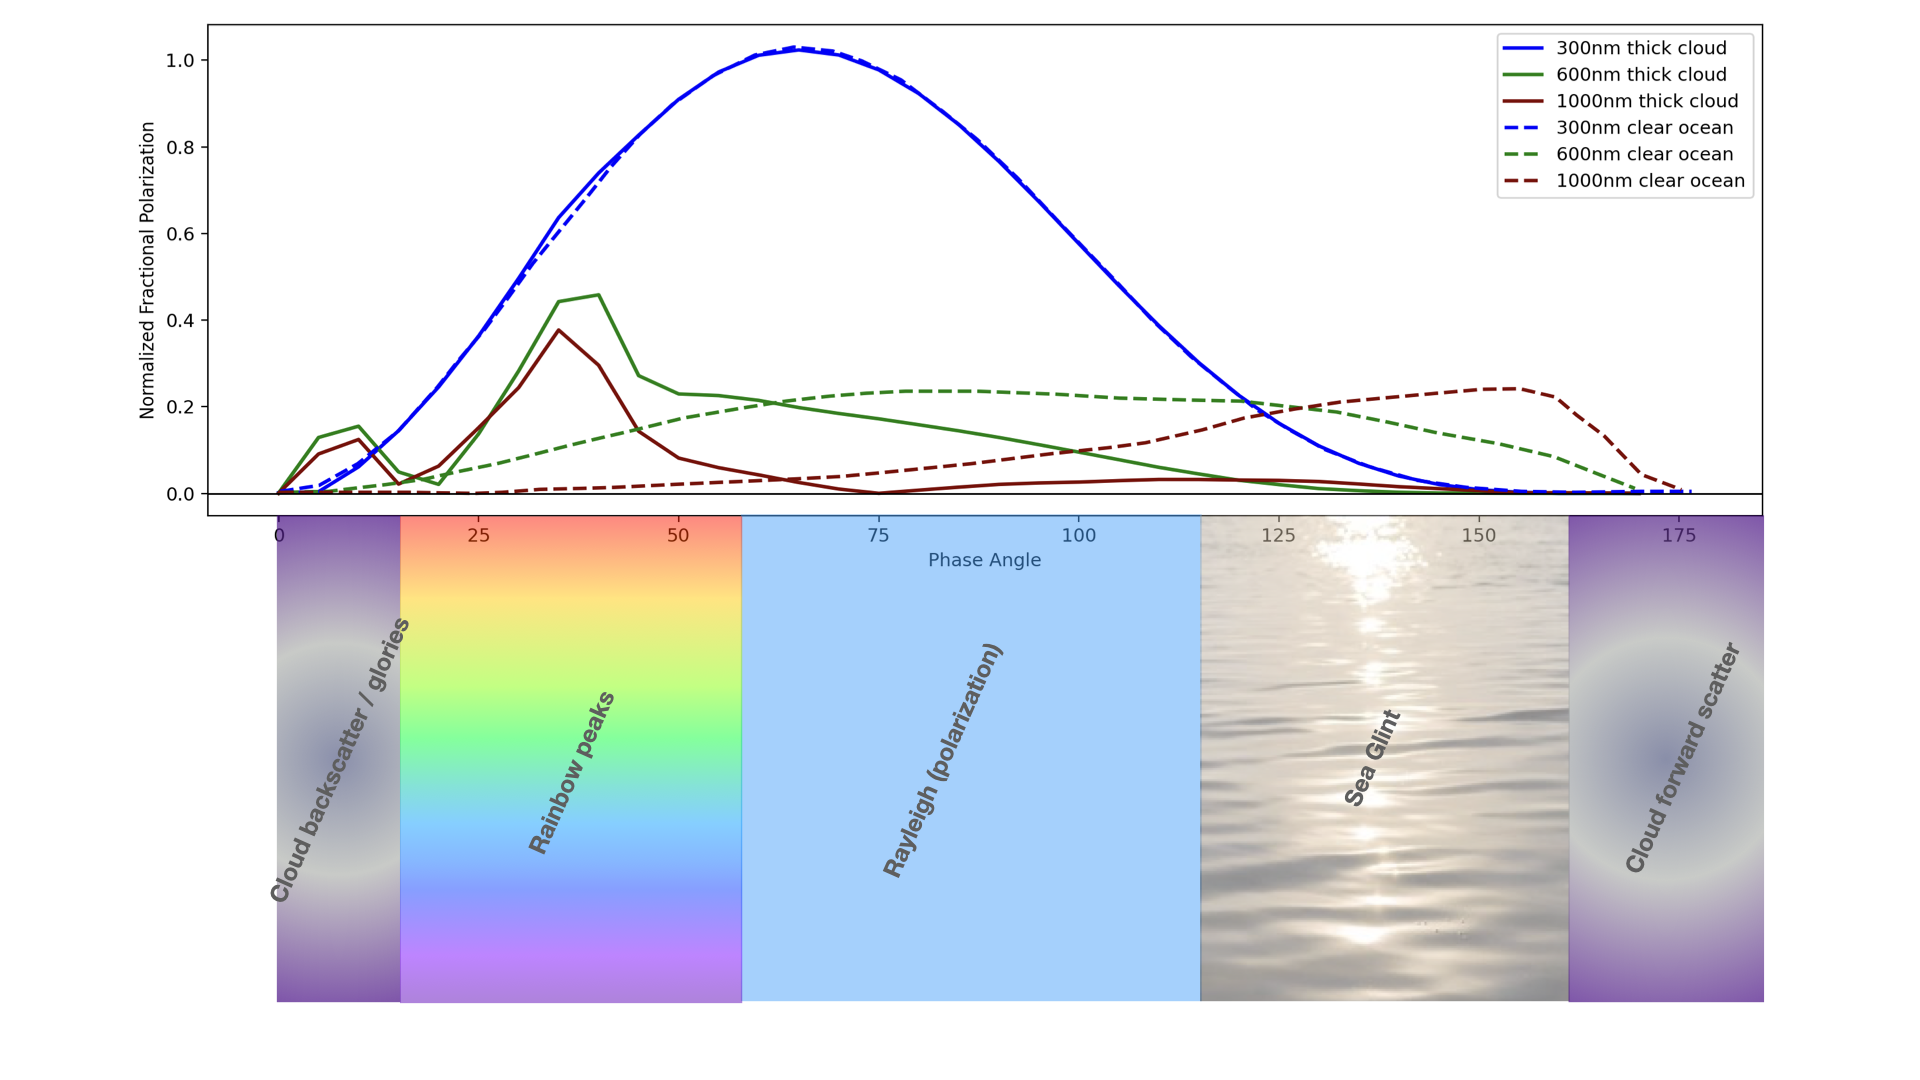
\includegraphics[width=\linewidth]{figures/Fig1IWAPol.png}
    \caption{
        The phase curves of two homogeneous planets with oceans and Earth-like atmospheres in edge-on orbits (the planets thus exhibit scattering angles 
        ranging from 0$^\circ$ to 180$^\circ$ along their orbits). 
        The cloudy scenario includes a low-altitude, Earth-like water 
        cloud deck. 
        Below the plot, we are showing the scattering angle ranges that cover the
        characteristic features of glories, rainbows, Rayleigh scattering, glint, and forward scattering by cloud particles (note that features partly overlap
        with each other).  
        Throughout the paper we approximate feature sensitivity ranges as those that capture the rise and fall of peaks in polarized light for most habitable zone species in the UV, Optical, and IR (phase angles: glint $\sim\qtyrange{50}{70}{\degree}$; rainbow $\sim\SIrange{140}{160}{\degree}$; Rayleigh narrow of quadrature, and other forward and backscattering effects at the widest and narrowest phase angles).
    }
    \label{fig:bottplot}
\end{figure*}


%--------------------------------------------------------------------------------

The field of exoplanet research has made great advances in the last few decades. The characterisation of Earth-like planets in the habitable zones of their stars is now at the frontier of what we can achieve. The Habitable Worlds Observatory will perform a dedicated direct imaging survey of nearby stars searching for rocky planets in the habitable zone. This space-based coronographic telescope will detect and characterise exoplanets using their reflection spectrum. Complementary information on the habitability of these worlds can be obtained by observing the change in the planet's brightness at different planetary phases.

Variations of the flux and in particular the degree of polarization of
light of the parent star that is reflected by an exoplanet as it moves
along its orbit that are due to an ocean glint or optical phenomena from scattering by condensates --- like the rainbow --- could be some of the most distinct signatures of habitability.
%
However, depending on the architecture of a planetary system, some of these features can be obscured by the inner working angle (\IWA{}) of a telescope's coronagraph.

Liquid surface water is closely related to planetary habitability because it is essential for life as we know it.
%
To first order, the presence of liquid surface water can be predicted by the flux a planet receives from its star.
%
The habitable zone (HZ) is defined as the range of semi-major axes around a given main sequence star for which a rocky planet (or moon) may have the right temperature to maintain liquid surface water \citep{kasting93}. 
%
However, there are many factors besides the incident stellar flux that influence a planet's surface temperature and ability to hold liquid surface water, such as the atmospheric surface pressure and, for example, geological activity. 
%
Establishing the presence of liquid surface water on an exoplanet would therefore provide important context for the interpretation of possible biosignatures.
%
Providing additional context to the habitability of an exoplanet would be the presence of a water cycle, as evidenced by the identification of a glint, i.e.\ the specular reflection of incident light by a liquid surface, or by a rainbow and other optical phenomena that can be attributed to light that is scattered by water clouds, as detailed in the next sections.

%The phase curves showing these features are distinct depending on the characteristics of the planet in both polarized and unpolarized measurements. Polarized and unpolarized phase curves and spectra each have their own strengths in characterization outlined below.

%%%%%%%%%%%%%%%%%%%%%%%%%%%%%%%%%%%%%%%%%%%%%%%%%%%%%%%%%%%%%%%%%%
\subsection{Exoplanet phase curves}

An exoplanet observed in an edge-on orbit will move through all phases and thus all phase angles, while those viewed at higher inclinations will pass through a subset of these phase angles.
%
If the planet is rotating, its reflected light signal in both total and polarized flux is expected to show temporal variations that can place constraints on the horizontal heterogeneity of the planet \citep{2001Natur.412..885F,stam2008,2022A&A...664A..59M}.

The strengths of detailed total and polarized flux phase curve analysis include mapping \citep{2001Natur.412..885F, berdyugina2019surface, 2022A&A...664A..59M}, the detection of dark areas or glint indicative of seas \citep{groot2020, cowan2008inverting, lustig2019}, and the characterization of clouds through forward- and back-scattering, rainbows, and glories.
%
An added potential benefit of observing the state of polarization of the reflected light is the suppression of starlight from quiescent stars without explicitly requiring a coronagraph or starshade as the light of these stars themselves can be considered to be unpolarized \citep{kemp1987}.

%%%%%%%%%%%%%%%%%%%%%%%%%%%%%%%%%%%%%%%%%%%%%%%%%%%%%%%%%%%%%%%%%%%

\subsection{Ocean glint}

%As ocean glint is one of the few sources of specular reflection and is strongly polarized, it provides one of the best means to detect a signature of habitability in exoplanet phase curves. 
Ocean glint is the specular (Fresnel) reflection of light off smooth liquid surfaces. While glint is a familiar phenomenon on Earth, there is only
one other body in the Solar System where it has been observed: 
the Cassini orbiter captured the glint of sunlight reflecting off the
liquid hydrocarbon lakes near Titan's north pole as it was observing
the moon from the nightside \citep{2010GeoRL..37.7104S}.
%
In the total flux, the glint signal is indeed expected to be most prominent at large planetary phase angles.
%
The maximum polarization occurs at the Brewster angle determined by the refractive indices at the interface; between air and liquid water this occurs at \qty{53}{\degree} \citep[i.e., a phase angle of \qty{127}{\degree}; see, e.g.,][]{2008Icar..195..927W}.
%
This angle therefore varies slightly with the wavelength and the composition of the ocean and the atmosphere.
%

In general, the glint on a planet will be strongest at red wavelengths where the Rayleigh scattering in the planet's atmosphere and attenuation through the atmosphere are smallest \citep{Zugger_2011} and, conveniently, where the latitude-albedo effect (a degeneracy between polar brightness and glint) is also small \citep{2012ApJ...752L...3C}.
%
The stronger glint signature at longer wavelengths has indeed been observed in Earthshine measurements \citep{Emde2017,sterzik2019, takahashi2021}.
%
The width across phase angles of the glint feature in total and polarized flux generally
broadens with increasing wave height \citep{kopparla2018, Zugger_2010, treesandstam2019, trees2022}, which depends strongly on the wind speed over the surface, as described by \citep{CoxMunk1954}.
%
{\color{red}{check the next sentence:}}
The broadening of the glint feature in the presence of wind-driven waves is well-described by the Cox-Munk solution \citep{CoxMunk1954}, shifts in both polarized and unpolarized light, and broadens across phase angles in polarized light \citep{kopparla2018, Zugger_2010, treesandstam2019, trees2022}. 

The glint provides evidence of liquid surface bodies, which, taken in the context of the temperature and types of condensates, may be interpreted as evidence for the presence of liquid water.
%
At large phase angles, the forward scattering of light by cloud particles could be confused with glint \citep{Robinson_2010}, which further motivated probing the rainbow angle for context.
%
This confusion can be solved by measuring the intersection of phase curves at various wavelengths in polarized light (the polarized colour changes from blue, through white, to red), which only occurs when the glint contributes to the signal and at a planetary scattering angle depending on the cloud coverage fraction \citep{treesandstam2019}.
%The cloud coverage fraction on ocean worlds could be constrained with observations spanning the ultraviolet to the near-infrared by finding the 
%angle at which the planet's polarization phase curves at various wavelengths intersect \citep{treesandstam2019}.
%
While the glint feature can only be probed when a planet is at crescent phases, \citet{trees2022} showed that reflection by a liquid surface body can also be detected with spectropolarimetry when the planet is at scattering angles where it is at the wide separations more easily probed when using coronagraphs.
%how use to map, 
%seen in Earthshine
%strong signal for exoplanets
% disentangled from cloud coupled with rainbow
%disentangled from lattitude albedo coupled in polarization

%%%%%%%%%%%%%%%%%%%%%%%%%%%%%%%%%%%%%%%%%%%%%%%%%%%%%%%%%%%%%%%%%%%%

\subsection{Rainbows, cloudbows and glories}

Rainbows, cloudbows, glories and other optical phenomena from light that is 
scattered by atmospheric condensates can dramatically influence the shape of a planet's total flux and polarized phase curves and provide a wealth of information 
about exoplanets \citep{karalidi2012rainbow, stam2008,Bailey2007,2014A&A...566L...1G}.%
\footnote{
    Rainbows occur when light is scattered by rain droplets that are large compared to the wavelength of the light. Cloudbows refer to features occurring at the same phase angles from smaller cloud particles with the spread in colors invisible to the human eye making them appear white \citet[see][for further discussion]{Bailey2007}.  
}
%
In our own Solar System, the polarized back scatter from Titan provided evidence that the moon's reflection was due to an atmospheric haze rather than a surface \citep{zellner1973polarization}, the polarized phase curve of Venus at three wavelengths showed not only that the clouds were $\sim\qty{75}{\percent}$ H\textsubscript{2}SO\textsubscript{4}--water mixture but also constrained the droplet size distribution \citep{hansenhovenier1974}. 
The glory feature in Venus's total flux phase curve was later used to rule out potential solutions for the unknown UV absorber \citep{petrova2018glory}.

In unpolarized light, the scattering by cloud particles can dramatically change the shape of a planet's phase curve compared to that of a 
Lambertian reflecting planet.
%
While the glory and rainbow are technically visible both in the total flux
and the polarized flux phase curves
in the presence of spherical cloud and/or haze particles, their strongly polarized nature coupled with the suppression of signals from other effects at gibbous and full phases in polarized light make them far easier to characterize in polarized flux than in total flux \citep{karalidi2011, stam2008, treesandstam2019}.
%
The rainbow angle depends on the refractive index of the scatterers and thus depends on their composition and the wavelength. 
The wavelength dependence itself also depends on the particles' size distribution, and the size distribution affects the angular shape of the rainbow \citep{karalidi2011}
%
Because the rainbow feature is narrower than the glint due to the surface reflection, it would 
allow for a more exact determination of the composition of the condensates.
%
Note that the scattering by clouds that consist of solid particles, 
such as ice crystals, will produce other optical features, such as halo's, particularly at small phase angles \citep{bailey2007, hansentravis1974, karalidi2012rainbow}.
%

In this paper, we define our optimal angle for the detection of a rainbow as that of the peak of the water droplet rainbow at visible wavelengths, which is around a phase angle $\alpha$ of 40$^\circ$ (see Fig.~\ref{fig:bottplot}).
%
Pushing observations to angles closer to the star (smaller phase angles, i.e., larger scattering angles) would allow the determination of the full shape of this rainbow, and enable the identification of rainbows due to the scattering of light by other possible HZ condensates.
%
The glory 
%is produced when the droplet radii much smaller than the wavelength of light 
can allow further characterization of condensates as its angle and shape also depend on the complex refractive index, but this feature occurs within \qty{20}{\degree} phase angle very close to full phase \citep{hansentravis1974}.
%
%The glory (in the backscattering direction) and diffraction peak (in the forward scattering direction) are distinct features in the total reflected flux, but not in the degree of polarization. In principle, the degree of polarization goes to zero in the forward and backward scattering directions. See e.g. Fig. 1 of \citet{stam2008}, Fig. 5 of \citet{trees2022}, Fig. 3 of \citet{karalidi2011} and \citet{hansentravis1974}.}}

\subsection{Habitable Worlds Observatory}

The National Academy of Sciences Astronomy \& Astrophysics 2020 Decadal Survey \citep{decadal} recommended the first in a new \enquote{Great Observatories} program, a telescope with the capability to detect signatures of habitability on about 25 HZ planets.
%
This requires an instrument with a coronagraph capable of high contrast imaging at optical to near infrared wavelengths.
%
Following the release of this survey, NASA recently announced the start of the development of the Habitable Worlds Observatory (\hwo).
%

The precursor technology recommended by the survey lists \enquote{direct imaging to probe polarized ocean glint on terrestrial planets} as one of the priority capabilities \citep[Box E.1 in][]{decadal} for ground and space-based observatories.
%
The performance and precise characteristics of \hwo{} (on-axis or off-axis, diameter, type of segmentation, type of coronagraph) are still to be determined.
%
The development will be heavily informed by the LUVOIR \citep{LUVOIR2019} and HabEx \citep{HabEx_2020} preparatory studies.
%
The Inner Working angle (\IWA{}) of the resulting telescope will depend on these characteristics, which in turn will have a significant impact on the expected exo-Earth yield \citep{Stark2019_exoplanetyield}.

The Extreme Coronagraph for Living Planetary Systems (ECLIPS) coronograph for LUVOIR was a proposed \qtyrange{200}{2000}{\nano\meter} instrument for exoplanet characterization, with a similar coronagraph, albeit operating between \num{450} and \qty{1800}{\nano\meter}, planned for HabEx.
%
POLLUX, a proposed instrument for LUVOIR would detect polarized light from hot Jupiters at \qty{300}{\nano\meter} \citep{Bouret2018_pollux}.
%
However, because of the challenges associated with the design of a coronagraph in the UV, it appears to be unlikely that \hwo{} will include a UV high-contrast instrument sensitive to Earth-like planets.

%We ignore contrast in this study
%OWA -> should go in discussions

%\textbf{In this paper we...}
\subsection{Outline}

In this paper, we quantify the planetary scattering angles that would be accessible for direct observations for hypothetical terrestrial planets orbiting in the habitable zones of \hwo{} target stars.
%
In \cref{subsec:2.1}, we describe the target list, in \cref{subsec:2.2} we derive expressions for the range of scattering angles given a few different limits, in \cref{subsec:2.3}, we describe Monte Carlo simulations to marginalize over the unknown orbital inclination and eccentricity of planets in these systems, and in \cref{subsec:2.4}, we outline how the planet/star contrast changes as a function of the planet's orbital phase.  
%
We present and discuss our results in \cref{sec:3}, and conclude in \cref{sec:4}. 
It is important to note that the phases angles selected for the features throughout this paper are approximate, that features overlap, and that their maximum peak will usually vary with chemical species and wavelength.

The conventions for angle names vary throughout the literature on exoplanet phase curves. In this paper we define the \textbf{scattering} angle as the local divergence in the light direction (large angles for back-scattering, small angles for forward-scattering); the \textbf{phase} angle $\varphi$ as the viewer-star-planet angle, which is zero at full phase and 180 at new phase, and which is the complement of the scattering angle. A planet with a face-on orbit will thus have a phase angle value of 90 degrees for the duration of its orbit.  In some plots we ``fold'' the half orbit so that we measure \textbf{degrees from quadrature} (so that both new and full phase are at maxima of 90$^\circ$ for edge on orbits), which is helpful in considering the visibility of the planet with inner working angle. We also note that we are considering here the polarization flux which takes into account the intensity of the polarization and reflectance (illumination) of the planet but additional information can be garnered from full Stokes characterization.

%the   the way that inclination and coronagraph inner working angle can limit the accessible scattering angles  
% We minimally explore the contrast ratio as we are primarily exploring whether these phase angles are reachable with inner working angle and outer working angle considered.

% We do not consider the particulars of specific planet scenarios as that work is completed by foward models

%We do not separate Stokes parameters as we are interested in where the net signal is achievable with IWA and OWA. 

%%%%%%%%%%%%%%%%%%%%%%%%%%%%%%%%%%%%%%%%%%%%%%%%%%%%%%%%%%%%%%%

%\section{Plots to Include}
%\label{sec:plots}
%\begin{enumerate}
%    \item \st{Cartoon defining various scattering angles: orbital phase, scattering phase, $\beta$ ? (Sophia)}
%    \item Bott plot: annotated polarized and unpolarized phase curves for ocean world and cloudy worlds (Kim)
%    \item \st{3x3 cartoon showing effect of inclination and IWA compared to orbit (Sophia)}
%    \item Cumulative distribution functions, both simple (circular, edge-on), bit more realistic (circular, but range of inclinations), and full-on (range of inclinations and eccentricities). Max \& Matthew
%    \item Scatter plot of stellar effective temperature vs system distance (Timmy)
%\end{enumerate}
 
%%%%%%%%%%%%%%%%%%%%%%%%%%%%%%%%%%%%%%%%%%%%%%%%%%%%%%%%%%%%%%%%%%%%%%%%%%%%%%%%%%%%%%%%%%%%%%%%%%%%%%%%%%%%%%%%%%%%%%%%%%%%%%

%\section{Observing scattering phenomena}
\section{Methods}

%%%%%%%%%%%%%%%%%%%%%%%%%%%%%%%%%%%%%%%%%%%%%%%%%%%%%%%%%%%%%%%

\subsection{\hwo{} and its stellar sample}
\label{subsec:2.1}

%\textcolor{blue}{Merge the 2 sections here into "Assumed technical specifications and sample"? I don't think this needs to be 2 subsections}
\hwo{} is still in the early stages of development, and although the exact telescope and instrument design have not yet been determined, we assume a \qty{6}{\meter} primary mirror, as suggested in The National Academy of Sciences Astronomy \& Astrophysics 2020 Decadal Survey.
%
The observatory will utilise a coronagraph to suppress the stellar light and facilitate high-contrast observations of faint accompanying exoplanets. 
%
The \IWA{} of the coronagraph will be driven by both the science requirements and technological limitations and is still unknown.
%In this work, we investigate the scattering phase coverage obtainable for several choices for the \IWA{} of the observatory. 
%We also consider the Outer Working Angle (OWA) but for most targets this is not a limiting factor. 
%From the HabWorlds report. Inner Working Angle: The IWA defines the region near the star that cannot be accessed for direct imaging due to a coronagraphic mask, starshade obscuration, or an interferometric null. It depends on the architecture of the telescope, the starlight suppression system used, and the observation wavelength. While a nominal value could be defined by making assumptions about the design for Habitable Worlds Observatory, we choose instead to derive the IWA from the star list itself and Astro2020’s requirement that ~100 cumulative habitable zones be surveyed by direct imaging. As shown in the main table, an IWA near ~70 mas will be needed to access ~100 cumulative habitable zones, and would need to be achieved at all wavelengths of interest for spectral characterization. For any specific telescope and starlight suppression system architecture the IWA is typically proportional to wavelength; thus, the number of accessible HZs will strongly decrease as IWA(lambda) increases.
For ease of comparison, \cref{tab:IWA_OWA} lists the angular separations corresponding to multiples of $\lambda / D$ for a \qty{6}{\meter} telescope at representative wavelengths $\lambda$ of $\qty{600}{\nano\meter}$ and $\qty{1}{\micro\meter}$.

%--------------------------------------------------------------------------
\begin{table}
    \centering
    \caption{
        Conversion between $\lambda / D$ and \unit{\mas} for wavelengths $\lambda$ of \qty{600}{\nano\meter} and \qty{1}{\micro\meter}, assuming the telescope's diameter $D$ is $\qty{6}{\meter}$ for the Inner and Outer Working Angles (i.e., the \IWA{} and \OWA{}, respectively). 
        %\todo{We should use consistent wavelengths for this table, for the Bott Plot, and for the M\&M cumulative distribution function. Also update to use the only wavelength we choose.}
    }
    \label{tab:IWA_OWA}
    \begin{tabular}{ c c c c } 
    \toprule
    & $\lambda/D$ & \unit{\mas} (at \qty{600}{\nano\meter}) & \unit{\mas} (at \qty{1}{\micro\meter}) \\
    \midrule
    \midrule
    IWA & 1 & 20.63 & 34.38 \\
    IWA & 2 & 41.25 & 68.75 \\
    IWA & 3 & 61.88 & 103.13 \\
    IWA & 4 & 82.51 & 137.51 \\
    \midrule
    OWA & 32 &  660.05 & 1100.08 \\
    OWA & 64 & 1320.09 & 2200.16 \\
    \bottomrule
    \end{tabular}
\end{table}
%--------------------------------------------------------------------------

\hwo{} is envisioned to observe the stars in the \emph{NASA Exoplanet Exploration Program's Mission Star List for the Habitable Worlds Observatory}.%
\footnote{Available online: \url{https://exoplanets.nasa.gov/internal_resources/2645_NASA_ExEP_Target_List_HWO_Documentation_2023.pdf}}
%
This list comprises $\sim\num{160}$ stars, the majority of which are Sun-like dwarfs: 66~F~dwarfs, 55~G~dwarfs, 40~K~dwarfs, and 3~M~dwarfs.
%
The target list is constructed assuming a maximum planet magnitude of $R_c = 31$ and a contrast floor of \num{2.5e-11}. 
%with an occurrence rate of rocky planets in the optimistic habitable zone to be $\eta_{\oplus}$ = 0.24 \citep{decadal}. 
The corresponding adopted habitable zone limits are a semi-major axis of \qtyrange{0.95}{1.67}{\au} for a solar twin, planet sizes between \qtyrange{0.8}{1.4}{} Earth radii, and for non-solar stars, scale as square root of the bolometric luminosity normalized to the Sun. 
%
This range of orbital separation corresponds to the \enquote{conservative habitable zone} \citep{kasting93, kopparapu13}. 
%
The authors of the Decadal Survey determined that for an imaging survey of habitable zones with a \qty{6}{\meter} telescope, these are the nearby stars (maximum distance \qty{25}{\parsec}) around which exo-Earths would be the best observable. 

In what follows, we consider hypothetical Earth-sized planets orbiting at the right distance from their parent star to receive the same flux as the Earth receives from the Sun.
%
By design, such planets should be observable by \hwo{} at least at their quadrature phase ($\alpha=90^\circ$).

%%%%%%%%%%%%%%%%%%%%%%%%%%%%%%%%%%%%%%%%%%%%%%%%%%%%%%%%%%%%%%%

\subsection{Maximum phase angle coverage}
\label{subsec:2.2}

A coronagraph can obscure part of the planet's orbit which, as shown in \cref{fig:annotated-orbit}, can prevent the planet from being observable at high and low phase angles. 
%
The range of observable phase angles will depend on the \IWA{} of the coronagraph, as well as on the orientation and shape of the exoplanet's orbit.

%--------------------------------------------------------------------------
% Figure 2
%--------------------------------------------------------------------------
\begin{figure}
    \centering
    \includestandalone{tikz/annotated-orbit}
    \caption{
        An illustration of a planet in an edge-on circular orbit showing how a coronagraph can obscure the exoplanet at high and low phase angles, and thus prevent observations of scattering features in an exoplanet's phase curve that could help to identify its atmospheric and/or surface composition and habitability. 
        The scattering angle, $\varphi$, is shown in red and is the complement of the phase angle in edge on systems.
    }
    \label{fig:annotated-orbit}
\end{figure}
%--------------------------------------------------------------------------

\subsubsection{Circular, edge-on orbits}

In the non-eccentric case (i.e., a circular orbit with the coronagraphic mask centred on the star), the minimum ($\varphi_\mathrm{min}$) and maximum ($\varphi_\mathrm{max}$) accessible phase angles are symmetric about 90$^\circ$. 
%
We define the angle $\Delta \varphi$ such that: 
\begin{equation}
 \label{eq:Delta_phi}
    \Delta \varphi 
    = \varphi_\mathrm{max} - \varphi_\mathrm{min}
    =  2 \cdot (\varphi_\mathrm{max} - \qty{90}{\degree}) 
    =  2 \cdot (\qty{90}{\degree} - \varphi_\mathrm{min} )  \,.
\end{equation} 
The on-sky projected planet distance, $r_\mathrm{proj}$ (in \unit{\au}) is shown in \cref{fig:scattering-angle} for a non-eccentric case with a 
semi-major orbital axis $a$ (in \unit{\au}), at a distance $d_*$ (in \unit{\parsec}) from the observer. 
%
The phase angle $\varphi$ is given by
\begin{equation}
    \sin(\varphi) = \frac{r_\mathrm{proj}}{a} \,.
    \label{eq:sinphi}
\end{equation}
%
Assuming small angles, $r_\mathrm{proj} = \delta d_*$ where $\delta$ is the on-sky angular separation.
%
We access the minimum phase angle when the projected distance reaches the inner working angle separation $\delta = \mathrm{IWA}$. 
%
Combining \cref{eq:Delta_phi} and \cref{eq:sinphi}, we deduce:
%
\begin{equation}
    \label{eq:scattering_angle}
    \cos\left(\dfrac{\Delta \varphi}{2}\right) = \frac{\mathrm{IWA} 
    \cdot d_*}{a} \,.
\end{equation}

%--------------------------------------------------------------------------
% Figure 3
%--------------------------------------------------------------------------
\begin{figure}
    \centering
    \includestandalone{tikz/scattering-angle}
    \caption{
        The on-sky projected planet distance, $r_\mathrm{proj}$, of a planet with a semi-major orbital axis $a$ at a distance $d_*$ from the observer.
        The on-sky angular separation as viewed by the observer is $\delta$.
        The phase angle, $\varphi$, is the angle between the line of sight to the star and the line connecting the star and planet.  
    }
    \label{fig:scattering-angle}
\end{figure}
%--------------------------------------------------------------------------

\Cref{fig:scatterplot} shows $\Delta \varphi$ for the systems in the \hwo{} target list, assuming an IWA of \qty{62}{\mas} ($3\,\lambda / D$ coronagraph at $\qty{600}{\nano\meter}$, see \cref{tab:IWA_OWA}). 
%
%This assumes each planet has a semi-major axis such that it receives an Earth-equivalent instellation, which is provided in the input star list.
%
As can be seen in \cref{fig:scatterplot}, for exoplanets in edge-on circular orbits, it will always be possible to observe the angular feature that is representative for Rayleigh scattering, as that occurs around quadrature ($\alpha=90^\circ$), while the rainbow angle (around $\alpha=40^\circ$) will only be accessible for a subset of exoplanets.

%--------------------------------------------------------------------------
% Figure 4
%--------------------------------------------------------------------------
\begin{figure*}
    \centering
    \includegraphics{figures/figure-4-scatterplot.pdf}
    \script{create-figure-4-scatterplot.py}
    \caption{
        Scatter plot for the target star sample, showing stellar effective 
        temperatures and distances.
        %
        The circle sizes represent the angular separation between 
        the star and its planet (in mas) as presented in the target list.
        %
        The colours show $\Delta \varphi$ assuming circular, edge-on orbits
        at a semi-major axis $a$ corresponding to an Earth-like 
        instellation and an IWA of \qty{62}{\mas}.
        %
        Additionally, the colour bar indicates the optical phenomena that 
        can in principle be detected: the phenomena from the bottom of the bar up to the colour of a given circle would be detectable for that planet.
        %
        For example, dark blue circles indicate planets on which most phenomena would be observable because planets that can be observed at the rainbow angle can also be observed at angles exhibiting Rayleigh scattering.
    }
    \label{fig:scatterplot}
\end{figure*}
%--------------------------------------------------------------------------

%%%%%%%%%%%%%%%%%%%%%%%%%%%%%%%%%%%%%%%%%%%%%%%%%%%%%%%%%%%%%%%%%%%%%%%%%%%

\subsubsection{Circular, inclined orbits}

Most planets are not in edge-on orbits as seen from Earth.
%
For an orbit with an inclination angle $i$, we can identify the following two regimes:% (see also \cref{fig:orb-grid}):
\begin{enumerate}
    \item The coronagraph does not obscure any part of the sky-projected orbit: 
    the maximum phase angle coverage depends solely on $i$. This 
    holds for orbits that are relatively face-on; 
    \item The coronagraph does obscure parts of the sky-projected orbit: 
    the phase angle coverage depends only on the \IWA{} and 
    the orbital semi-major axis $a$. 
\end{enumerate}

%--------------------------------------------------------------------------
% Figure 5
%--------------------------------------------------------------------------
\begin{figure}
   \centering
   \includegraphics[width=0.99\columnwidth]{figures/figure-5-orb-grid.pdf}
   \script{create-figure-5-orb-grid.py}
   \caption{
        The phase angles accessible to a direct imaging mission 
        can be limited by either the orbital inclination angle $i$ or the coronagraphic \IWA{}.
        %
        If the orbit is close to face-on (top panels), the phase angles probed along the orbit are limited by the inclination angle $i$; for circular orbits, the accessible scattering phases are $\phi \in \qty{90}{\degree} \pm i$. 
        %
        For orbits close to edge-on (bottom panels) the planet attains all 
        phases, but the phase angles near \qty{0}{\degree} and \qty{180}{\degree} are not observable due to obscuration by the coronagraph; for circular orbits, the accessible scattering phases are $\phi \in \qty{90}{\degree} \pm \arcsin({\rm IWA}\cdot d_*/a)$.
    }
    \label{fig:orb-grid}
\end{figure}
%--------------------------------------------------------------------------

Using \cref{eq:scattering_angle}, we deduce the following for inclined 
circular orbits: 
\begin{equation}
\label{eq:Delta_phi_max}
    \Delta \varphi = 
    \begin{cases}
        2 i & \textrm{for} \cos(i) > \frac{\mathrm{IWA}\; d_* }{a} \\ 
        2 \cos^{-1}\left(\dfrac{\mathrm{IWA}\cdot d_* }{a}\right) & \textrm{for} \cos(i) < \frac{\mathrm{IWA}\; d_* }{a}
    \end{cases} \,.
\end{equation}

%%%%%%%%%%%%%%%%%%%%%%%%%%%%%%%%%%%%%%%%%%%%%%%%%%%%%%%%%%%%%%%

%\subsubsection{Eccentric orbits}

%The inclination $i$ is sampled such that $\cos(i)$ follows a uniform distribution, $\cos(i) \sim \mathcal{U}(0, 1)$.

%%%%%%%%%%%%%%%%%%%%%%%%%%%%%%%%%%%%%%%%%%%%%%%%%%%%%%%%%%%%%%%%%%%%%%%%%%%

\subsection{Monte Carlo simulations}
\label{subsec:2.3}

\subsubsection{Circular, randomly inclined orbits}
\label{sec:circular}

For each star on the \hwo{} target list, we generate \num{1000} random orbits of hypothetical habitable planets in orbits with semi-major axes that yield an Earth-equivalent-incident stellar flux. 
%
The orbital inclination angles $i$ are randomly drawn from a distribution 
that is uniform in $\cos i$. 
%
We then use \cref{eq:Delta_phi_max} to determine the range of 
accessible phase angles for each hypothetical planet.
%
The solid lines in \cref{fig:betaallofit} show the cumulative 
distribution of the maximum and minimum accessible phase 
angles normalised to the total number of systems in the \hwo{} 
target list for different values of the \IWA{}.

%%%%%%%%%%%%%%%%%%%%%%%%%%%%%%%%%%%%%%%%%%%%%%%%%%%%%%%%%%%%%%%%%%%%%%%%%%%

%--------------------------------------------------------------------------
\begin{figure*}%[t]
    \centering
    \includegraphics[width=0.95\textwidth]{figures/figure-6-n-over-phase.pdf}
    \script{create-figure-6-n-over-phase.py}
    \caption{
        The cumulative distributions of the most extreme phase angles accessible for different \IWA{} and for randomly inclined, circular orbits
        (solid lines) and randomly inclined, elliptical orbits (dashed lines).
        %
        The top $x$-axis indicates the minimum and the 
        bottom $x$-axis the maximum accessible phase angle.
        %
        These angles are symmetric about quadrature (90 degrees).
        %
        The $y$-axis on the left indicates the number of planetary systems 
        divided by the number of Monte Carlo samples and is thus normalised to 
        the number of systems on the target list.
        %
        The $y$-axis on the right indicates the number of systems, assuming \qty{24}{\percent} of them have an Earth-like planet in their HZ.
    }
    \label{fig:betaallofit}
\end{figure*}
%--------------------------------------------------------------------------

%%%%%%%%%%%%%%%%%%%%%%%%%%%%%%%%%%%%%%%%%%%%%%%%%%%%%%%%%%%%%%%%%%%%%%%%%%%
\subsubsection{Eccentric, randomly inclined orbits}
\label{sec:eccentric}

We repeat the Monte Carlo simulations from \cref{sec:circular} assuming 
the orbital eccentricity follows a beta-distribution with shape parameters 
$a=0.867$ and $b=3.03$ \citep{2013MNRAS.434L..51K}. 
%
We randomly draw \num{1000} orbits for each star and determine the sky-projected orbits following, for example, \citet{2010exop.book...15M}. 
Orbital eccentricities are drawn from the beta distribution, and 
inclination angles are uniform in $\cos i$. 
\Cref{fig:ball-o-yarn} shows a sample of the generated orbits.
%

We then calculate the minimum and maximum accessible phase 
angles for \IWA{}s of \qtylist{21; 42; 63; 84}{\mas} which correspond to 1, 2, 3 and 4 times $\lambda / D$ at $\qty{600}{\nano\meter}$, respectively (see \cref{tab:IWA_OWA} and the dashed lines in \Cref{fig:ball-o-yarn}).
%
The dashed lines in \cref{fig:betaallofit} show the normalised cumulative 
distribution of the accessible phase angles for each value of the 
\IWA{} for eccentric orbits. 
%
We also calculate which target planets would be observable at the phase angles where ocean glint, rainbows, or the Rayleigh peak occur.
%
The cumulative distribution over the \IWA{} of the number of planetary systems where all optical phenomena would be observable, normalised to the total number of systems, is shown in \cref{fig:accessible_phase_angles}.
%

%%%%%%%%%%%%%%%%%%%%%%%%%%%%%%%%%%%%%%%%%%%%%%%%%%%%%%%%%%%%%%%%%%%%%%%%%%%
\subsection{Simulating contrast curves}
\label{subsec:2.4}

A second parameter that is crucial for detecting angular features like 
rainbows and ocean glint on Earth-like exoplanets is the contrast, i.e.\ 
the ratio of the flux of the starlight that is reflected by the planet 
and the direct stellar flux. 
%
While this is not the main focus of this paper, it is important to consider that the total flux contrast and the polarized contrast generally 
depend on the phase angles, due to a combination of the changing illumination fraction of the observable planetary disk and the non-isotropic reflection by the planet.
%
Here, we aim to present some simplified examples of the impact of the 
phase angle dependent contrast on the detectability of rainbow and 
glint features. 
%
We note that these calculations are by no means complete or exact, given 
the many variables that go into the modelling of reflected total and
polarized fluxes of Earth-like exoplanets \citep{ treesandstam2019,trees2022}.
%

The NASA Exoplanet Exploration Program’s Mission Star List for \hwo{} 
includes for every star an estimated contrast for an Earth-twin in 
the habitable zone.
%
% The cited paper has all the equations that lead to this equation:
The contrast is given by \citep[see, e.g.,][]{2023A&A...671A.165M}
\begin{equation}
    C(\alpha) 
    = F_p(\alpha) / F_* 
    = A_\mathrm{G} \cdot \phi(\alpha) \cdot \left( R_p / a(\alpha) \right)^2 \,,
\label{eq:contrast}
\end{equation}
where $A_\mathrm{G}$ is the planet's geometric albedo, $R_p$ its radius, $\phi(\alpha)$ is the integral phase function at scattering angle $\alpha$
(normalized to \num{1.0} at full phase), and $a$ is the distance between the planet and its host star.
\todo{here, $\alpha$ is used for the scattering angle ... and is the 
'integral phase function' the same as the 'scattering phase function'?}
%
The assumptions that went into the contrast estimations for \hwo{}
are that $a$ is constant (the orbits are thus circular), the geometric albedo $A_{\rm G}$ is \num{0.2}, and that the phase function, $\phi(\alpha)$, can be described by a simple Lambertian reflectance phase function, which assumes isotropic reflection by the planetary surface.
%
These calculations give an order-of-magnitude calculation for the 
contrast of Earth-like planets around nearby stars.
%
Therefore, in this work, we will assume that the calculated contrasts 
in the list correspond to the reflected flux at quadrature and normalize the phase functions to this point.
%
We do not aim to accurately calculate the absolute scaling of the contrast, as this depends on many factors and would have required some work for the star list to be redone.
%

We use the phase functions from \citet{treesandstam2019} 
for an Earth-like planet with an ocean surface with a wind-speed of $\qty{7}{\meter\per\second}$ at $\qty{670}{\nano\meter}$ and covered by patchy clouds.
%
The $\qty{670}{\nano\meter}$ is close to the centre of the Rc band for Vega ($\qty{642}{\nano\meter}$). 
%
We normalize the phase function at quadrature and multiply it with the 
contrast.
%
In addition, we map the orbital phase for circular orbits to the phase angle and the on-sky separation given an inclination of \num{90} degrees.
%
Together, they give the reflected light contrast as a function of separation for a full orbit.
%
We multiply this flux with the degree of polarization and retrieve the polarized contrast.
%
The resulting contrast curves are shown in \cref{fig:contrasts} for 
three of the closest target stars: the G~dwarf $\alpha$~Cen~A, the K~dwarf 
$\epsilon$~Eri, and the M~dwarf Lalande~21185.

%--------------------------------------------------------------------------
\begin{figure*}%[t]
   \centering
   \includegraphics[width=0.99\textwidth]{figures/figure-7-contrast-over-separation_i=90.pdf}
    \script{create-figure-7-contrast-over-separation.py}
   \caption{
    The contrast (Eq.~\ref{eq:contrast}) and orbital separation 
    of an Earth-like planet with an ocean surface and patchy clouds 
    along its orbit with an assumed inclination angle $i$ of \qty{90}{\degree} around $\alpha$~Cen~A, $\epsilon$~Eri, and Lalande~21185.
    %
    The solid, black line indicates the contrast in unpolarized light, 
    with the contrast at quadrature marked by the black dot.
    %
    The polarized component is indicated by the coloured dots, with the colour representing the phase angle from quadrature.
    %
    The light grey dots show the contrasts at quadrature of the other targets in the star list, and the dashed lines indicate $1$, $2$ and $3$ times the \IWA{} for \hwo.
    }
    \label{fig:contrasts}
\end{figure*}
%--------------------------------------------------------------------------

%%%%%%%%%%%%%%%%%%%%%%%%%%%%%%%%%%%%%%%%%%%%%%%%%%%%%%%%%%%%%%%%%%%%%%%%%%%
\section{Results}
\label{sec:3}

%\todo{Is there a plot for this? How many systems could we see? Why is it different to non-eccentric cases?}
%\timmy{No plot / results yet; see above.}
%\todo{Sophia: what is features\_plot\_peak.png showing?}
%\timmy{Good question --- maybe Matt or Max know how the data for this was generated? Matt: yes, it's all in showyourwork right now. I ran 1000 sims for each target with a random eccentric orbit, then pulled out the betamax and betamin angles for each of the 1000 realisations. Max's plots encode the completeness as a function of scattering angle, showing that you get about 10 percent more phenomena. }

%%%%%%%%%%%%%%%%%%%%%%%%%%%%%%%%%%%%%%%%%%%%%%%%%%%%%%%%%%%%%%%

\subsection{The effect of eccentricity}
\label{sec:result_eccentricity}

As shown in \cref{fig:betaallofit}, allowing the planet's orbit to be eccentric can have a noticeable effect on the number of systems that can be observed at each phase angle.
%
This is because---as Kepler's second law explains---eccentric planets spend more time at orbital separations greater than their semi-major axis, and hence are more likely to peak out from behind the coronagraph \IWA{} and extreme orbital phases (albeit with worse contrast due to the greater star-planet separation).
%
The eccentricity does not significantly affect the number of systems for \IWA{} smaller than cut used in the selection of the systems in the \hwo{} target list. 
It is, however, important to account for orbital eccentricity when the \IWA{} of the coronagraph is larger than the \IWA{} used to filter the target list; otherwise, the number of systems observable at extreme scattering angles would be under-predicted.

%%%%%%%%%%%%%%%%%%%%%%%%%%%%%%%%%%%%%%%%%%%%%%%%%%%%%%%%%%%%%%%

\subsection{Observable optical phenomenon}
\label{sec:results_scattering_phenomena}

In this section, we consider the number of stars around which different optical phenomena could be observable for different \IWA{}.
%
We first define the scattering angles over which various of these phenomena are accessible in \cref{tab:phase_ranges}.
%
We note that these ranges should all be considered approximate, as the exact scattering angles where these phenomena are dominant depend on the details of the atmospheric and surface properties, as well as the wavelengths being observed.
%
Nonetheless, this exercise can provide valuable insights on the effects of \IWA{} choice. 

\Cref{fig:accessible_phase_angles} shows the number of systems in which key scattering phenomena will be observable for different \IWA{}.
%
The \IWA{} of \hwo's coronagraph will depend on the primary mirror diameter, observing wavelength, and how well a coronagraph of a given size can suppress the glare of the host star.
%
The smaller the \IWA{}, the more features we will be observable and in more systems. 

%--------------------------------------------------------------------------
%--------------------------------------------------------------------------
\begin{table}
    \centering
    \caption{
        The approximate ranges of scattering angles for the different optical phenomena considered in this paper.
    }
    \label{tab:phase_ranges}
    \begin{tabular}{ l c c c } 
        \toprule
        & $\varphi_\mathrm{min}$ & $\varphi_\mathrm{peak}$ & $\varphi_\mathrm{max}$ \\
        \midrule
        \midrule
        Rainbow    & 22$^\circ$    & 42$^\circ$    & 63$^\circ$ \\
        Rayleigh    & 50$^\circ$    & 70$^\circ$    & 110$^\circ$ \\
        Ocean Glint & 130$^\circ$   & 150$^\circ$   & 170$^\circ$ \\
        Glory       & 0$^\circ$     & 5$^\circ$     & 10$^\circ$ \\
        \bottomrule
    \end{tabular}
\end{table}
%--------------------------------------------------------------------------
    % features = {r'Rainbow': (127,138,158),
    %         r"Rayleigh": (90,110,130),
    %         r"Ocean Glint": (50,30,10),
    %         r"Glory": (10,5,0),
    %         }

The Rayleigh feature, which can be used to determine if a planet has an atmosphere, appears near quadrature and is therefore observable in the most systems.
%
The rainbow feature appears further from quadrature (around $\alpha=40^\circ$), but will still be observable in a significant fraction of systems.
%
The position and shape of the rainbow peak is sensitive to the properties of the droplets, allowing their nature to be determined if the peak of the rainbow feature can be reached.
%
The ocean glint feature occurs even further from quadrature and so would be observable in fewer systems. 
%
In most systems, only the first half of the glint feature would be observable, but this can still be used to identify a liquid ocean on the surface of a planet.
%
A key indicator of habitability. 
Finally, it is possible to view the glory scattering feature in one system, Alpha~Cen~A.

%--------------------------------------------------------------------------
%--------------------------------------------------------------------------
\begin{table}
    \centering
    \caption{
        Number of stars around which the peak scattering angle of each phenomenon is detectable, expressed in \unit{\mas} and $\lambda/D$ for $\lambda = \qty{600}{\nano\meter}$ and $D = \qty{6}{\meter}$.
    }
    \label{tab:nstars_detect}
    \begin{tabular}{ l c c c } 
        \toprule
        & \multicolumn{3}{c}{IWA}\\
        & \qty{21}{\mas} & \qty{41}{\mas} & \qty{62}{\mas} \\
        & $2\,\lambda/D$ & $3\,\lambda/D$ & $4\,\lambda/D$\\
        \midrule
        \midrule
        Rainbows    & 90  & 42    & 18 \\
        Rayleigh    & 152 & 115   & 65 \\
        Ocean Glint & 43  & 14    & 5 \\
        % Glory       & 0   & 5     & 10 \\
        \bottomrule
    \end{tabular}
\end{table}
%--------------------------------------------------------------------------

%%%%%%%%%%%%%%%%%%%%%%%%%%%%%%%%%%%%%%%%%%%%%%%%%%%%%%%%%%%%%%%

\subsection{Contrast curves}
\label{sec:results_contrast}

The accessible phase angle is not the only factor that needs to be considered when determining what scattering features are observable.
%
The contrast of the planet is also an important factor to consider.
%
\Cref{fig:contrasts} shows approximate contrast curves for three of the stars in the \hwo{} target list assuming edge-on orbits.
%
The overall contrast varies significantly for each system and throughout the orbit.
%
The observability of these planets will depend on the starlight suppression of the coronagraph, which is influenced by its \IWA{}.
%
It is not possible to predict how much the state of the art of coronagraphy will have advanced by the time \hwo{} is built.
%
However, when its design is being finalised, it will be important to consider both the accessible phase angles and contrast limits when deciding on the \IWA{} of the coronagraph, if these features are to be observed.

%%%%%%%%%%%%%%%%%%%%%%%%%%%%%%%%%%%%%%%%%%%%%%%%%%%%%%%%%%%%%%%

%--------------------------------------------------------------------------
% Figure 8:
%--------------------------------------------------------------------------
\begin{figure*}
    \centering
    \includegraphics{figures/figure-9-yarnball.pdf}  
    \script{create-figure-8-yarnball.py}
    \caption{
        Examples of the eccentric orbits generated for the stellar sample.
        %
        The orbits are scaled by the Earth-equivalent incident flux distance. 
        %
        The concentric, dashed circles indicate \IWA{}s of \num{20.6}, \num{41.3}, \num{61.9}, and \qty{82.5}{\mas}, corresponding to 1, 2, 3, and 4\,$\lambda / D$, respectively (assuming $\lambda = \qty{600}{\nano\meter}$ and $D = \qty{6}{\meter}$).
        %
        Each system has been scaled such that its HZ has the same radius, 
        hence the variation in the size of the \IWA{}s compared to the orbits.
        It is clear that the \IWA{} can significantly affect the range of 
        observable scattering phases for each orbit.
    }
    \label{fig:ball-o-yarn}
\end{figure*}
%--------------------------------------------------------------------------

%--------------------------------------------------------------------------
% Figure 9:
%--------------------------------------------------------------------------
\begin{figure*}
    \centering
    \includegraphics{figures/figure-9-n-over-iwa.pdf}
    \script{create-figure-9-n-over-iwa.py}
    \caption{
        The number of systems for which key optical phenomena (Rayleigh scattering, rainbow, ocean glint, glories) would be observable as functions of the \IWA.
        %
        Each subplot contains three lines showing the number of systems where the start of the phenomena is observable (dashed lines), where the peak is observable (solid lines), and where the end is observable (dotted lines).
        %
        The $x$-axis at the bottom shows the \IWA{} of the coronagraph in \unit{mas}, and the $x$-axis at the top shows the same \IWA{} converted to $\lambda/D$ for $\lambda = \qty{600}{\nano\meter}$ and $D = \qty{6}{\meter}$.
        %
        The $y$-axis on the right indicates the number of systems where 
        all phenomena would be observable, assuming \qty{24}{\percent} of them have an Earth-like exoplanet in their HZ.
        %
        It is worth noting that the Glory would be observable in only one system: Alpha~Cen~A.
    }
    \label{fig:accessible_phase_angles}
\end{figure*}
%--------------------------------------------------------------------------

%%%%%%%%%%%%%%%%%%%%%%%%%%%%%%%%%%%%%%%%%%%%%%%%%%%%%%%%%%%%%%%%%%%%%%%%%%%

\section{Conclusions}
\label{sec:4}

%What did we determine? 
%Can we actually detect this stuff for anything in this sample? 
%Do we need to not something about things like A stars which are not included in the sample - they were rejected by the list creators - do we need to comment on this?  - we decided nope.

The Habitable Worlds Observatory is a coronagraphic space telescope 
envisioned to detect and characterize Earth-like exoplanets in the 2040's. 
%
The instrument design and capabilities are still under development and 
should be driven by the mission's science goals.
%
In this work, we investigated the possibility of using \hwo{} to detect optical phenomena with specific angular features in polarized reflected light, such as rainbows, ocean glint, and glory's, which could establish a planet's habitability. 
%
We primarily focused on the range of accessible phase angles given the limitations of the coronagraphic \IWA{} and aimed to investigate which phenomena could potentially be observed.
%
Coronagraphy is a rapidly advancing field, and it is hard to predict what the capabilities of \hwo{} will be.
%
The desire to detect and characterize a large number of Earth-like exoplanets, and the intrinsic occurrence of such planets, will drive the choice of coronagraphic \IWA{} for this mission.
%
Assuming a \qty{62}{\mas} \IWA{}, all \num{160} planetary systems in the NASA Exoplanet Exploration Program's Mission Star List for \hwo{} would be observable at scattering phases where angular features due to Rayleigh scattering show up, but the rainbow of light that is scattered in droplets of water clouds would only be accessible in $\sim\num{42}$ systems, and ocean glint in $\sim\num{14}$ systems.
%
The habitability of Earth-like exoplanets in the remaining 146 systems would have to be established through less direct methods like rotational mapping to identify horizontally inhomogeneous surface coverage, for example due to presumably bright continents and dark oceans \citep[e.g.,][]{2009ApJ...700..915C,lustig2019}.   
%
The fraction of habitable zones around stars in the target list that can be probed by \hwo{} increases with decreasing \IWA{}. 
%
Additionally, decreasing the \IWA\ also increases the range of scattering angles observable in these systems. 
%
Therefore, to increase the number of systems for which key features such as ocean glint can be observed, the primary mirror diameter could be increased and/or the \IWA of the coronagraph could be decreased.
%
While we briefly considered the contrast ratio of the scattering features, we did not investigate the feasibility of detecting them given their contrast. 
%
This will be an important task once the instrument design and capabilities are better defined and could drive the design of the coronagraph and the primary mirror diameter. 

%\todo{the paragraph below seems similar to the one above ... merge them?}
%We have shown that with a \qty{6}{\meter} primary mirror and a coronagraph with an \IWA\ of $3\,\lambda/D$ at \qty{600}{\nano\meter}, only $\sim\qty{10}{\percent}$ of the Earth-like exoplanets targeted by \hwo{} would be observable at a range of scattering angles that is wide enough to establish the presence of liquid surface water via the polarization signature of the glint (i.e., specular reflection).  
%
%This number could be improved by increasing the primary mirror diameter or decreasing the \IWA of the coronagraph.
%
%While we briefly considered the contrast ratio of the scattering features, we did not investigate the feasibility of detecting them given their contrast. 
%
%This will be an important task once the instrument design and capabilities are better defined and could drive the design of the coronagraph and the primary mirror diameter. 

%%%%%%%%%%%%%%%%%%%%%%%%%%%%%%%%%%%%%%%%%%%%%%%%%%%%%%%%%%%%%%%%%%%%%%%%%%%
\section*{Software/Data Availability}

\todo{check the naming and references/footnotes for this list throughout the paper}
The NASA ExEP target list containing the data used for these simulations is  available online.%
\footnote{\url{https://exoplanets.nasa.gov/exep/science-overview/}}
This work has made use of \textsf{numpy}
 \citep{NumPy2020}, \textsf{scipy} \citep{scipy_2020}, \textsf{matplotlib} \citep{matplotlib2007}, and \textsf{astropy},\footnote{\url{https://www.astropy.org}} a community-developed core Python package and an ecosystem of tools and resources for astronomy \citep{astropy:2013, astropy:2018, astropy:2022}.

%%%%%%%%%%%%%%%%%%%%%%%%%%%%%%%%%%%%%%%%%%%%%%%%%%%%%%%%%%%%%%%%%%%%%%%%%%%
\section*{Acknowledgements}

%The workshop on which this manuscript is based was made possible thanks to the logistical and financial support of the Lorentz Center, Leiden, Netherlands.
%
%This workshop was supported by NOVA  and by the European Research Council (ERC) under the European Union's Horizon 2020 research and innovation programme (grant agreement No. 866001 - EXACT).
%
%This research has made use of NASA's Astrophysics Data System Bibliographic Services and the SIMBAD database, operated at CDS, Strasbourg, France. 
%
%SRV acknowledges funding from the European Research Council (ERC) under the European Union’s Horizon 2020 research and innovation program under grant agreement No 805445.
%
%SLC acknowledges support from an STFC Ernest Rutherford Fellowship. 
%
%TDG acknowledges funding from the Max Planck ETH Center for Learning Systems.
%
%Specific grant funding and any other specific requirements
%
%KMB acknowledges support from NASA Habitable
%
%Worlds grant No. 80NSSC20K152, and previous support for related work supported by NASA Astrobiology Institute's Virtual Planetary Laboratory under Cooperative Agreement Number NNA13AA93A.
%
%This paper has been formatted in the {\tt showyourwork!} framework, which includes the computer code to reproduce the figures, including the associated data, within an online repository to make it reproducible \citep{Luger2021}.

The Optimal Exoplanet Imaging workshop (2023) on which this manuscript is based was made possible thanks to the logistical and financial support of the Lorentz Center, Leiden, The Netherlands. 
%
The research presented in this paper was initiated at a workshop held in Leiden and partially supported by NOVA (the Netherlands Research School for Astronomy) and by the European Research Council (ERC) under the European Union's Horizon 2020 research and innovation programme (grant agreement n°866001 - EXACT).

This research has made use of NASA's Astrophysics Data System Bibliographic Services and the SIMBAD database, operated at CDS, Strasbourg, France. 

SRV acknowledges funding from the European Research Council (ERC) under the European Union’s Horizon 2020 research and innovation program under grant agreement No 805445.
SLC acknowledges support from an STFC Ernest Rutherford Fellowship. 
TDG acknowledges funding from the Max Planck ETH Center for Learning Systems.
KMB acknowledges support from NASA Habitable Worlds grant No. 80NSSC20K152, and previous support for related work from NASA Astrobiology Institute's Virtual Planetary Laboratory under Cooperative Agreement Number NNA13AA93A.
ILa acknowledges the support by a postdoctoral grant issued by the Centre National d'Études Spatiales (CNES) in France.
PBa, ILa, and YGu were supported by the Action Spécifique Haute Résolution Angulaire (ASHRA) of CNRS/INSU co-funded by CNES.
EHP is supported by the NASA Hubble Fellowship grant \#HST-HF2-51467.001-A awarded by the Space Telescope Science Institute, which is operated by the Association of Universities for Research in Astronomy, Incorporated, under NASA contract NAS5-26555.
L.A. and E.C. acknowledge funding from the European Research Council (ERC) under the European Union's Horizon Europe research and innovation programme (ESCAPE, grant agreement No. 101044152).
O.A. and L.K. acknowledge funding from the European Research Council (ERC) under the European Union’s Horizon 2020 research and innovation programme (grant agreement No 819155)
SYH was funded by the generous support of the Heising-Simons Foundation.
RJP is supported by NASA under award number 80GSFC21M0002.

This paper has been formatted in the {\tt showyourwork!} framework, which includes the computer code to reproduce the figures, including the associated data, within an online repository to make it reproducible \citep{Luger2021}.

%%%%%%%%%%%%%%%%%%%%%%%%%%%%%%%%%%%%%%%%%%%%%%%%%%%%%%%%%%%%%%%%%%%%%%%%%%%

% \clearpage

% References
\bibliographystyle{mnras}
\bibliography{bib}

%%%%%%%%%%%%%%%%%%%%%%%%%%%%%%%%%%%%%%%%%%%%%%%%%%%%%%%%%%%%%%%%%%%%%%%%%%%
\section*{Author affiliations}
\begingroup
    \itshape
    \raggedright
    \affdest{1}Department of Astrophysics, University of Oxford, Denys Wilkinson Building, Keble Road, Oxford OX1 3RH, UK \\[0.5mm]
    \affdest{2}Department of Earth and Planetary Sciences, University of California, Riverside, CA 92521, USA \\[0.5mm]
    \affdest{3}NASA Nexus for Exoplanet System Science, Virtual Planetary Laboratory Team, Seattle, WA 98195, USA \\[0.5mm]
    \affdest{4}NASA Nexus for Exoplanet System Science, Terrestrial Polarization Team, Orlando, FL 32826, USA \\[0.5mm]
    \affdest{5}Centre for Exoplanet Research, School of Physics and Astronomy, University of Leicester, University Road, Leicester, LE1 7RH, UK \\[0.5mm]
    \affdest{6}Department of Earth \& Planetary Sciences and Department of Physics, McGill University, 3600 rue University, Montréal, QC, H3A 2T8, Canada \\[0.5mm]
    \affdest{7}Leiden Observatory, Leiden University, P.O. Box 9513, 2300 RA Leiden, The Netherlands \\[0.5mm]
    \affdest{8}SRON Netherlands Institute for Space Research, Niels Bohrweg 4, 2333 CA, Leiden, The Netherlands \\[0.5mm]
    \affdest{9}Max Planck Institute for Intelligent Systems, Max-Planck-Ring 4, 72076 Tübingen, Germany \\[0.5mm]
    \affdest{10}ETH Zurich, Institute for Particle Physics \& Astrophysics, Wolfgang-Pauli-Str. 27, 8092 Zurich, Switzerland \\[0.5mm]
    \affdest{11}LESIA, Observatoire de Paris, Université PSL, CNRS, Sorbonne Université, Université de Paris, 92195 Meudon, France \\[0.5mm]
    \affdest{12}Department of Physics, University of California, Santa Barbara, CA 93106, USA \\[0.5mm]
    \affdest{13}STAR Institute, Université de Liège, Allée du six Août 19c, 4000 Liège, Belgium \\[0.5mm]
    \affdest{14}Aix Marseille Univ, CNRS, CNES, LAM, Marseille, France \\[0.5mm]
    \affdest{15}NASA Ames Research Center, Bldg. 245, Moffett Field, USA \\[0.5mm]
    \affdest{16}Université Grenoble Alpes, CNRS, IPAG, 38000 Grenoble, France \\[0.5mm]
    \affdest{17}Department of Astronomy, California Institute of Technology, Pasadena, CA, 91125, USA \\[0.5mm]
    \affdest{18}University of California, Santa Cruz, USA \\[0.5mm]
    \affdest{19}DTIS, ONERA, Université Paris Saclay, 91123 Palaiseau, France \\[0.5mm]
    \affdest{20}DOTA, ONERA, 92322 Châtillon, France \\[0.5mm]
    \affdest{21}Steward Observatory, University of Arizona, 933 North Cherry Avenue, Tucson, AZ 85719, USA \\[0.5mm]
    \affdest{22}Subaru Telescope, NAOJ, USA \\[0.5mm]
    \affdest{23}College of Optical Sciences, University of Arizona, Tucson, AZ 87521, USA \\[0.5mm]
    \affdest{24}Astrobiology Center, 2 Chome-21-1, Osawa, Mitaka, Tokyo, 181-8588, Japan \\[0.5mm]
    \affdest{25}NASA Goddard Space Flight Center, 8800 Greenbelt Rd, Greenbelt, MD  20771, USA \\[0.5mm]
    \affdest{26}University of Maryland Baltimore County, 1000 Hilltop Cir, Baltimore, MD 21250, USA \\[0.5mm]
    \affdest{27}European Space Agency, ESTEC, Keplerlaan 1, 2200 AG Noordwijk, The Netherlands \\[0.5mm]
    \affdest{28}Université Côte d'Azur, Observatoire de la Côte d'Azur, CNRS, Laboratoire Lagrange, France \\[0.5mm]
    \affdest{29}Space Telescope Science Institute, 3700 San Martin Drive, Baltimore, MD 21218, USA \\[0.5mm]
    \affdest{30}Delft University of Technology, Kluyverweg 1, 2629 HS Delft, The Netherlands \\[0.5mm]
    \affdest{31}Department of Geoscience \& Remote Sensing, Delft University of Technology, Stevinweg 1, 2628 CN, Delft, The Netherlands \\[0.5mm]
    \affdest{32}Royal Netherlands Meteorological Institute (KNMI), Utrechtseweg 297, 3731 GA, de Bilt, The Netherlands \\[0.5mm]
    \affdest{33}National Research Council Canada, Herzberg Astronomy and Astrophysics Research Center, Victoria, B.C., Canada \\[0.5mm]
\endgroup

%%%%%%%%%%%%%%%%%%%%%%%%%%%%%%%%%%%%%%%%%%%%%%%%%%%%%%%%%%%%%%%%%%%%%%%%%%%
\end{document} 